\chapter{Quantitative analysis of injection beam loss}\label{sec:Quantitative analysis of injection beam loss}

\section{Collimator offset study}
\subsection{Motivation}


\subsection{D02V1 collimator}

\begin{figure}
    \centering
    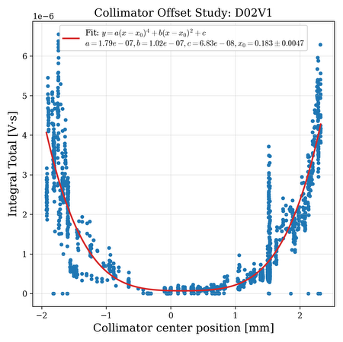
\includegraphics[width=0.6\columnwidth]{Figures/C05_Quantitative_analysis/Offset/D02V1.png}
    \caption{CLAWS sensor}
    \label{fig:CLAWS}
\end{figure}
\begin{figure}
    \centering
    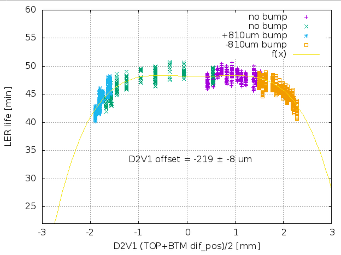
\includegraphics[width=0.6\columnwidth]{Figures/C05_Quantitative_analysis/Offset/D02V1_life.png}
    \caption{CLAWS sensor}
    \label{fig:CLAWS}
\end{figure}


\subsection{D03V4 collimator}

\begin{figure}
    \centering
    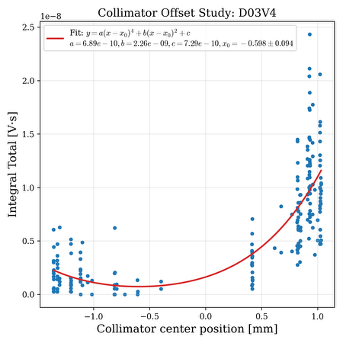
\includegraphics[width=0.6\columnwidth]{Figures/C05_Quantitative_analysis/Offset/D03V4.png}
    \caption{CLAWS sensor}
    \label{fig:CLAWS}
\end{figure}
\begin{figure}
    \centering
    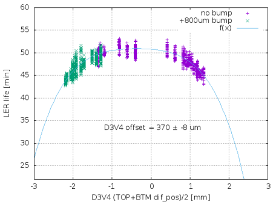
\includegraphics[width=0.6\columnwidth]{Figures/C05_Quantitative_analysis/Offset/D03V4_life.png}
    \caption{CLAWS sensor}
    \label{fig:CLAWS}
\end{figure}



\subsection{D01V1 collimator}

\begin{figure}
    \centering
    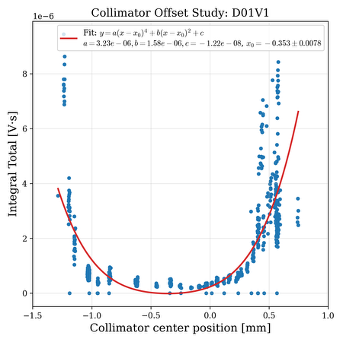
\includegraphics[width=0.6\columnwidth]{Figures/C05_Quantitative_analysis/Offset/D01V1.png}
    \caption{CLAWS sensor}
    \label{fig:CLAWS}
\end{figure}
\begin{figure}
    \centering
    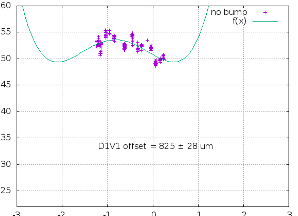
\includegraphics[width=0.6\columnwidth]{Figures/C05_Quantitative_analysis/Offset/D01V1_life.png}
    \caption{CLAWS sensor}
    \label{fig:CLAWS}
\end{figure}